\documentclass[12pt]{article}

\usepackage{sbc-template}
\usepackage{graphicx}
\usepackage{url}
\usepackage[brazil]{babel} 
\usepackage[utf8]{inputenc}
\usepackage{booktabs}
\usepackage[pdftex]{hyperref}
\usepackage{indentfirst}
\usepackage{float}

     
\sloppy

\title{MangueSMART: Sistema de Apoio à Decisão para o Planejamento Urbano Inteligente de Aracaju}

\author{Beathriz Laurent Carlos Muniz\inst{1}, Jeferson de Oliveira Santos\inst{2}, \\João Marcos Peixoto Cavalcante\inst{3}, Marcelo Pedral Mota\inst{4}, \\Niceu Santos Biriba\inst{5}, Gilton José Ferreira da Silva\inst{2} } 

\address{Departamento de Computação (DCOMP)\\ Universidade Federal de Sergipe
  (UFS)\\
  Av. Marechal Rondon, s/n -- Jardim Rosa Elze -- CEP 49100-000 \\São Cristóvão -- SE -- Brazil
  \email{beathriz.muniz@dcomp.ufs.br, jeferson.santos@dcomp.ufs.br}
  \email{joao.cavalcante@dcomp.ufs.br, marcelo.mota@dcomp.ufs.br}
  \email{niceu.biriba@dcomp.ufs.br, gilton@dcomp.ufs.br}
}

\begin{document} 

\maketitle

\begin{abstract} \textbf{Context:} Aracaju's rapid urban expansion demands data-driven planning for socio-environmental sustainability. \textbf{Objective:} This study develops and validates MangueSMART, a Decision Support System (DSS) prototype for smart urban planning. \textbf{Method:} The approach integrates urban data (ETL) using the 4+1 View Model and Project Model Canvas. \textbf{Results:} The system enables scenario simulations and integrated dashboards, optimizing analysis time for public managers. \textbf{Conclusions:} MangueSMART aligns local policies with smart city guidelines, fostering inclusive and sustainable governance. \end{abstract}
     
\begin{resumo} \textbf{Contexto:} A expansão urbana de Aracaju exige um planejamento estruturado e orientado por dados para assegurar a sustentabilidade. \textbf{Objetivo:} Este trabalho desenvolve e valida o MangueSMART, um protótipo de Sistema de Apoio à Decisão (SAD) para o planejamento urbano inteligente. \textbf{Método:} Utilizou-se integração de dados (ETL), arquitetura Visão-Modelo 4+1 e Project Model Canvas. \textbf{Resultados:} O sistema provê dashboards e simulações de cenários, otimizando o tempo de análise técnica dos gestores. \textbf{Conclusões:} A solução alinha a gestão de Aracaju às diretrizes de cidades inteligentes e governança sustentável. \end{resumo}

\section{Introdução} \label{sec:introducao}
O projeto MangueSMART surge em um cenário onde o município de Aracaju apresenta um crescimento urbano acelerado, resultando em desafios significativos de acessibilidade, mobilidade e infraestrutura. Atualmente, a gestão urbana enfrenta dificuldades devido à fragmentação de dados entre departamentos e à carência de ferramentas integradas que apoiem a tomada de decisão estratégica. Para mitigar esses problemas, este trabalho propõe a adoção do Project Model Canvas como instrumento de planejamento, visando a criação de um Sistema de Apoio à Decisão (SAD) que articule indicadores urbanos e simulações de desenvolvimento.


\subsection{Justificativa}
\label{sec:justificativa}
% --- SEÇÃO 1.1 ---
O município de Aracaju enfrenta um cenário de crescimento urbano acelerado, caracterizado pela verticalização intensa em áreas centrais e pela expansão da malha urbana periférica, muitas vezes associada a assentamentos informais. Conforme aponta o Observatório das Metrópoles \cite{observatorio2023}, esse dinamismo impõe desafios complexos à gestão pública, resultando na saturação da infraestrutura e mobilidade deficiente.

Além disso, iniciativas recentes buscam mitigar o déficit habitacional, como a destinação de áreas da União para regularização fundiária \cite{agenciagov2025} e projetos de revitalização do centro urbano \cite{govse2025}. No entanto, o processo decisório ainda enfrenta obstáculos significativos devido à fragmentação de dados entre diferentes secretarias e à carência de ferramentas analíticas integradas.

A relevância do projeto \textit{MangueSMART} reside na mudança de paradigma para o conceito de cidades inteligentes, onde o planejamento deixa de ser reativo para se tornar orientado por dados (\textit{data-driven}). Segundo Iwasa \cite{iwasa2025}, o planejamento estratégico é vital para a efetivação dessas tecnologias. A implementação de um Sistema de Apoio à Decisão (SAD) justifica-se pela necessidade de articular indicadores de uso do solo e mobilidade, alinhando a administração pública a diretrizes de sustentabilidade e justiça urbana \cite{rdc2024}.

\section{Objetivos} 
O objetivo geral deste trabalho é desenvolver e validar um protótipo funcional, especificamente um Produto Mínimo Viável (MVP), de um Sistema de Apoio à Decisão (SAD) denominado MangueSMART. O foco do sistema é o planejamento urbano inteligente da cidade de Aracaju, integrando dados para permitir a simulação de cenários de uso do solo e mobilidade, visando reduzir o tempo de análise técnica de gestores públicos e promover a sustentabilidade socioambiental.

\section{Benefícios} 

O principal benefício do \textit{MangueSMART} é a entrega de um protótipo funcional de Sistema de Apoio à Decisão que centraliza dados urbanos dispersos. A literatura destaca que cidades inteligentes sustentáveis dependem de estratégias de implementação que integrem tecnologia e gestão \cite{rdc2024}. Espera-se reduzir drasticamente o tempo de análise técnica para aprovação de projetos e definição de políticas públicas. A longo prazo, o sistema visa alinhar o planejamento de Aracaju aos princípios de governança digital e eficiência, conforme discutido nas revisões sobre planejamento de \textit{Smart Cities} \cite{iwasa2025}.

\section{Descrição das próximas seções} 
O trabalho está estruturado da seguinte forma: a Seção \ref{sec:oque} detalha o produto, os trabalhos relacionados e as visões arquiteturais (lógica, desenvolvimento, processo e física). A Seção \ref{sec:quem} apresenta a equipe e a persona do cliente-alvo. A Seção \ref{sec:Como} descreve a metodologia, premissas e entregas. A Seção \ref{sec:quandoquanto} aborda o cronograma e os custos. Por fim, as Seções \ref{sec:ameacas} e \ref{sec:consideracoes} discutem as limitações do projeto e apresentam as considerações finais.

\section{O que será feito?} \label{sec:oque}

\subsection{Produto}

O \textbf{MangueSMART} é um protótipo funcional (MVP) de um Sistema de Apoio à Decisão (SAD) voltado ao planejamento urbano inteligente de Aracaju (SE). A solução consiste em uma plataforma digital que integra camadas de dados urbanos padronizadas e dashboards temáticos focados em uso do solo, mobilidade e infraestrutura. O objetivo é permitir que gestores monitorem indicadores e analisem cenários para promover uma cidade mais sustentável e inclusiva.

\subsection{Trabalhos Relacionados}

A literatura sobre Aracaju revela diagnósticos setoriais críticos: Teixeira et al. (2023) apontam a subutilização de vazios urbanos centrais; Meneses et al. (2024) destacam os riscos de inundação agravados pela desatualização do Plano Diretor ; e Santos e Pinto (2020) demonstram o surgimento de ilhas de calor devido ao adensamento construtivo.

No campo tecnológico, a plataforma "AjuInteligente" é criticada por ser meramente administrativa, carecendo de inteligência analítica para o planejamento urbano. Embora esses estudos ofereçam dados precisos, há uma carência de ferramentas que integrem essas informações heterogêneas. O MangueSMART supre essa lacuna ao propor um SAD que cruza indicadores de uso do solo, riscos ambientais e mobilidade, permitindo a simulação de cenários futuros para o suporte à decisão estratégica.
\subsection{Arquitetura Visão-Modelo 4+1}

\subsubsection*{Visão Lógica}

Diagrama de classes:

\begin{figure}[H]
\centering
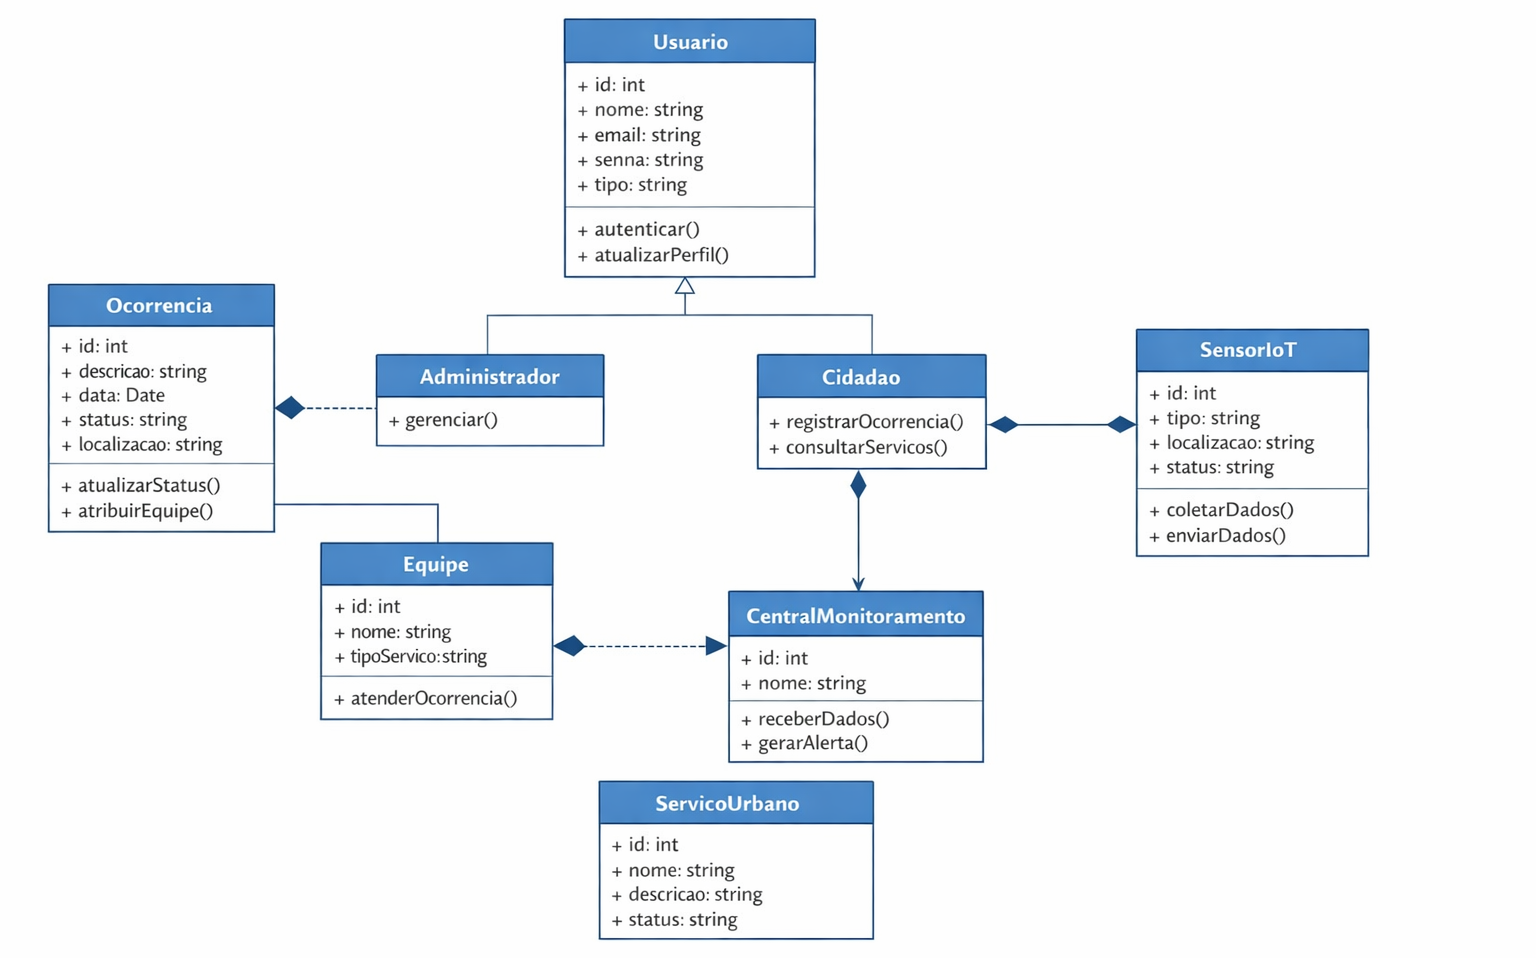
\includegraphics[width=0.9\textwidth]{images/diagramas/diagrama_de_classes.png}
\label{fig:diagrama_de_classes}
\end{figure}

\subsubsection*{Visão de Desenvolvimento}

Diagrama de componentes:

\begin{figure}[H]
\centering
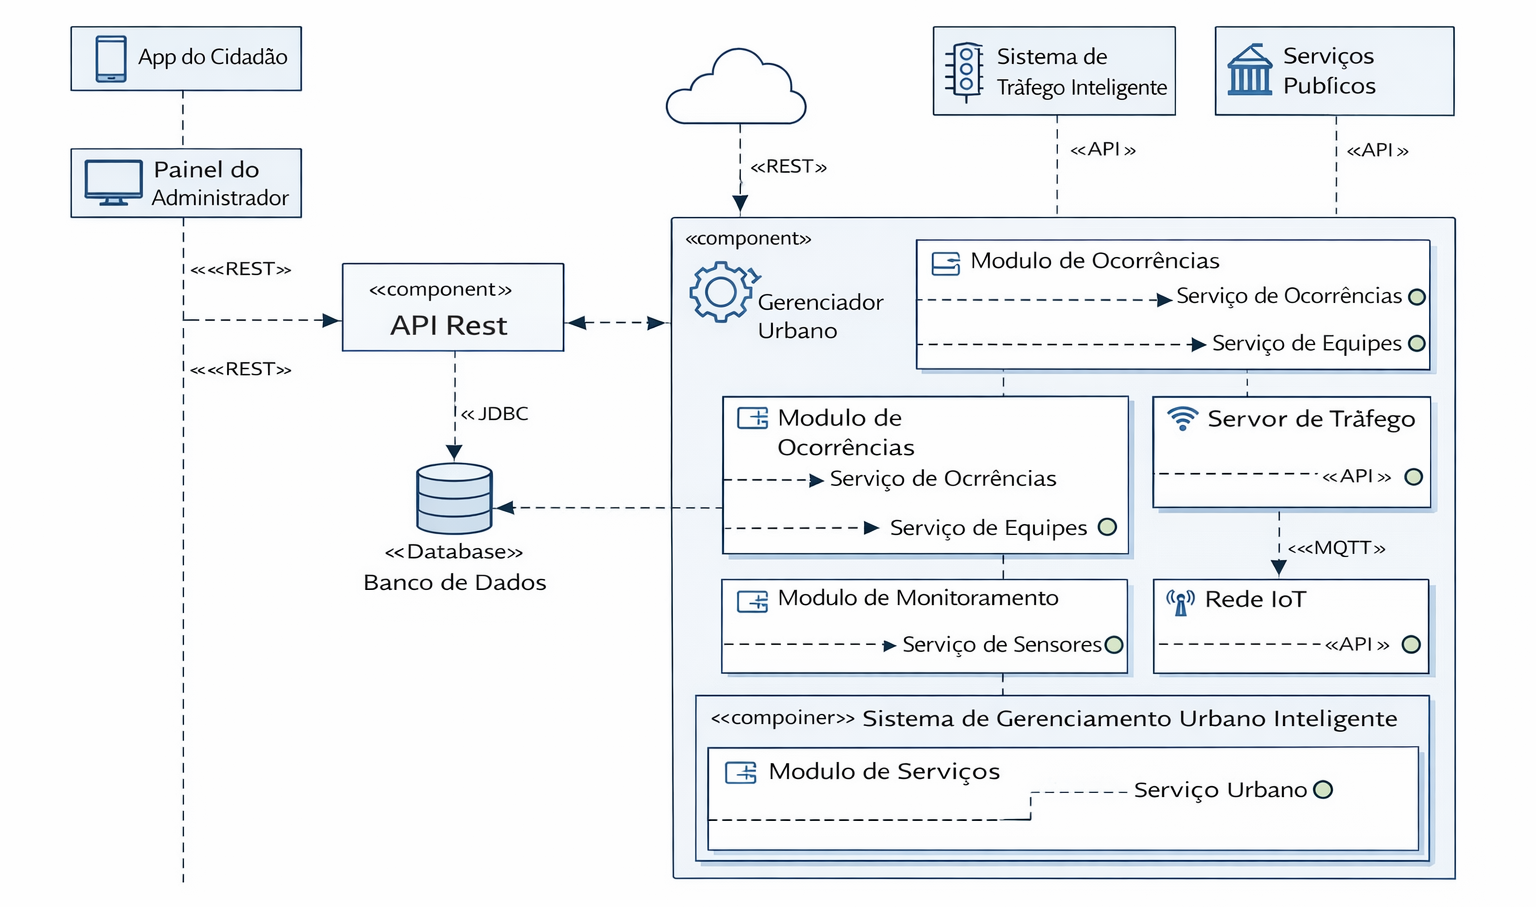
\includegraphics[width=0.9\textwidth]{images/diagramas/diagrama_de_componentes.png}
\label{fig:diagrama_de_componentes}
\end{figure}


\subsubsection*{Visão de Processo}

Diagrama de atividades:

\begin{figure}[H]
\centering
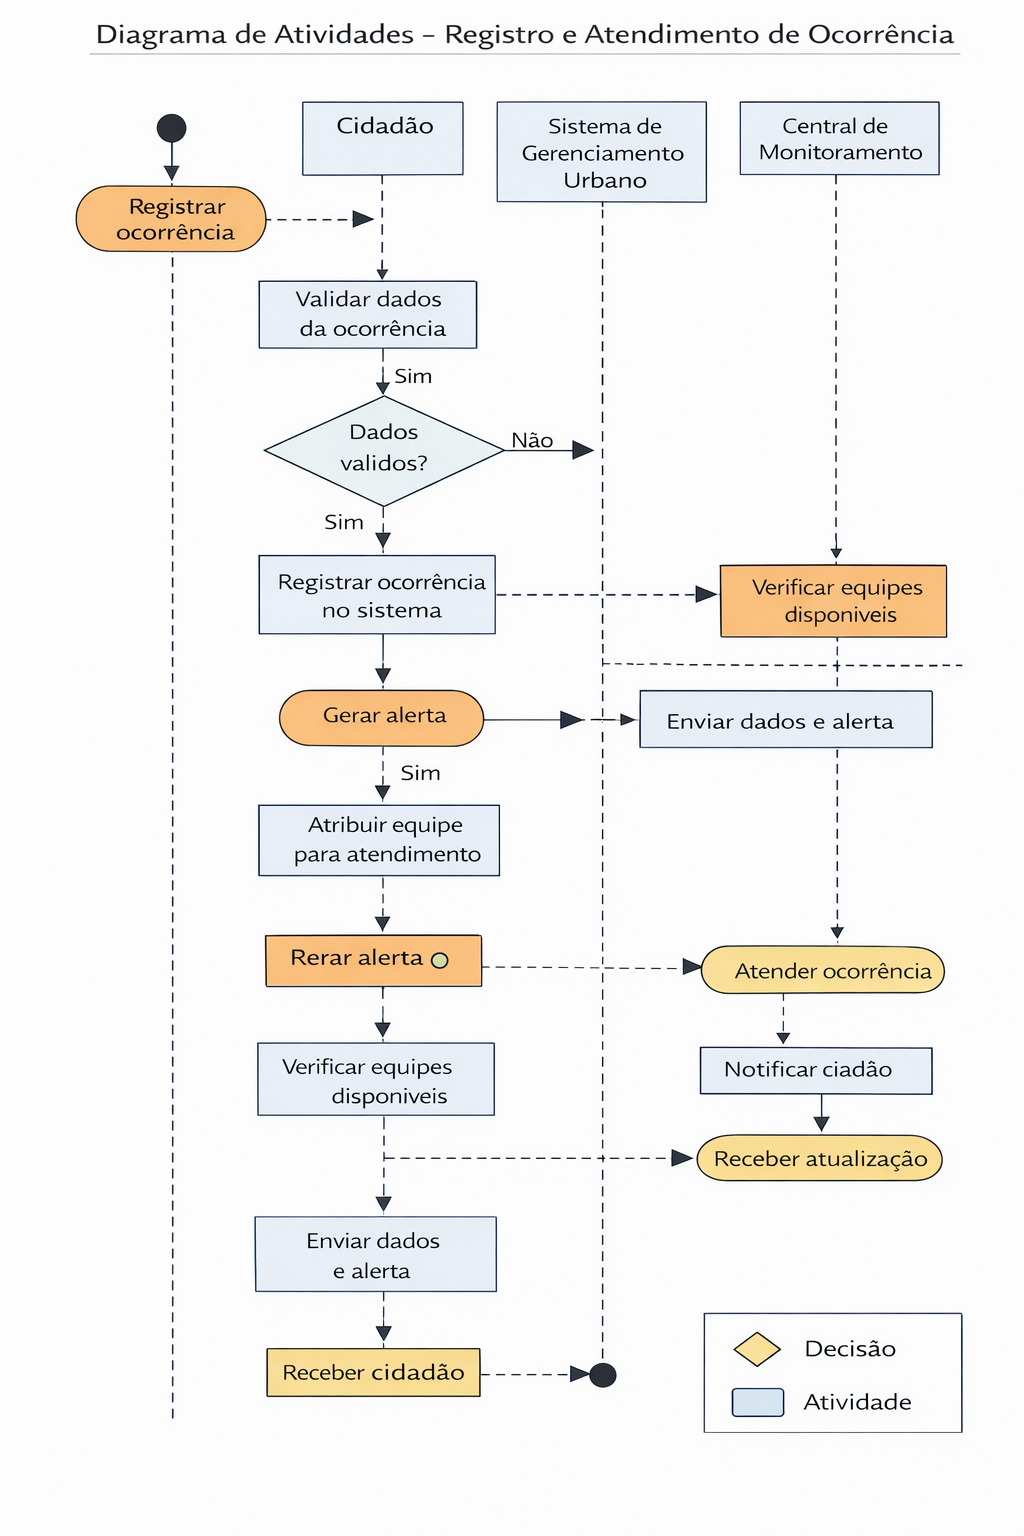
\includegraphics[width=0.8\textwidth]{images/diagramas/diagrama_de_atividades.png}
\label{fig:diagrama_de_atividades}
\end{figure}

\subsubsection*{Visão Física}

Diagrama de Implantação:

\begin{figure}[H]
\centering
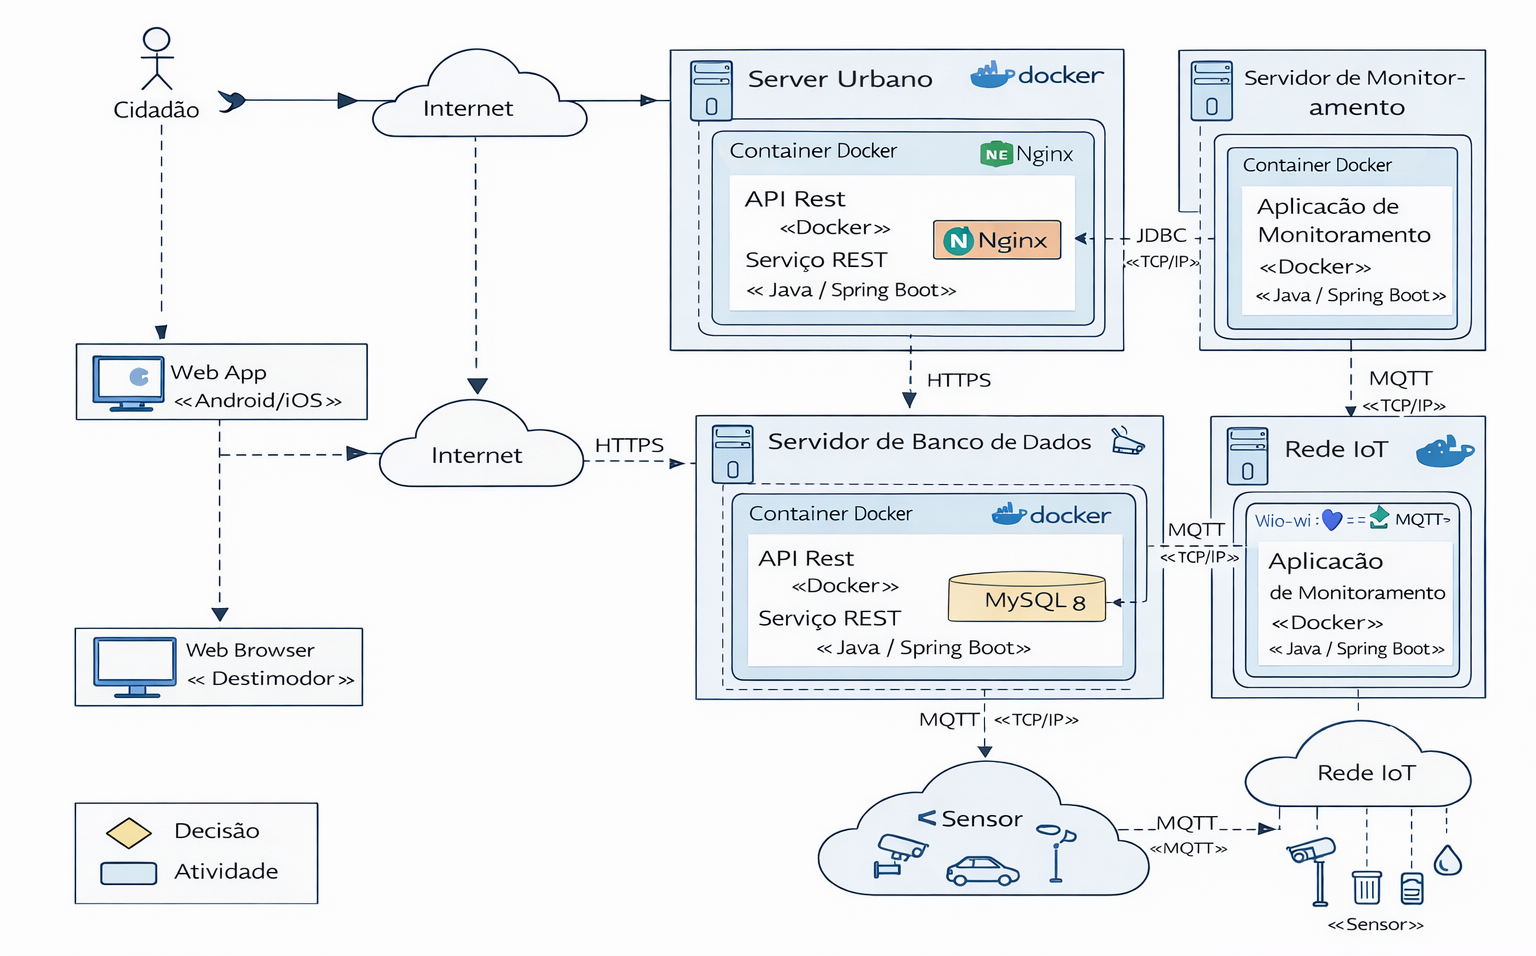
\includegraphics[width=0.9\textwidth]{images/diagramas/diagrama_de_implantacao.png}
\label{fig:diagrama_de_implantacao}
\end{figure}

\subsubsection*{Visão de Caso de Uso}

Diagramas de Casos de Uso:

\begin{figure}[H]
\centering
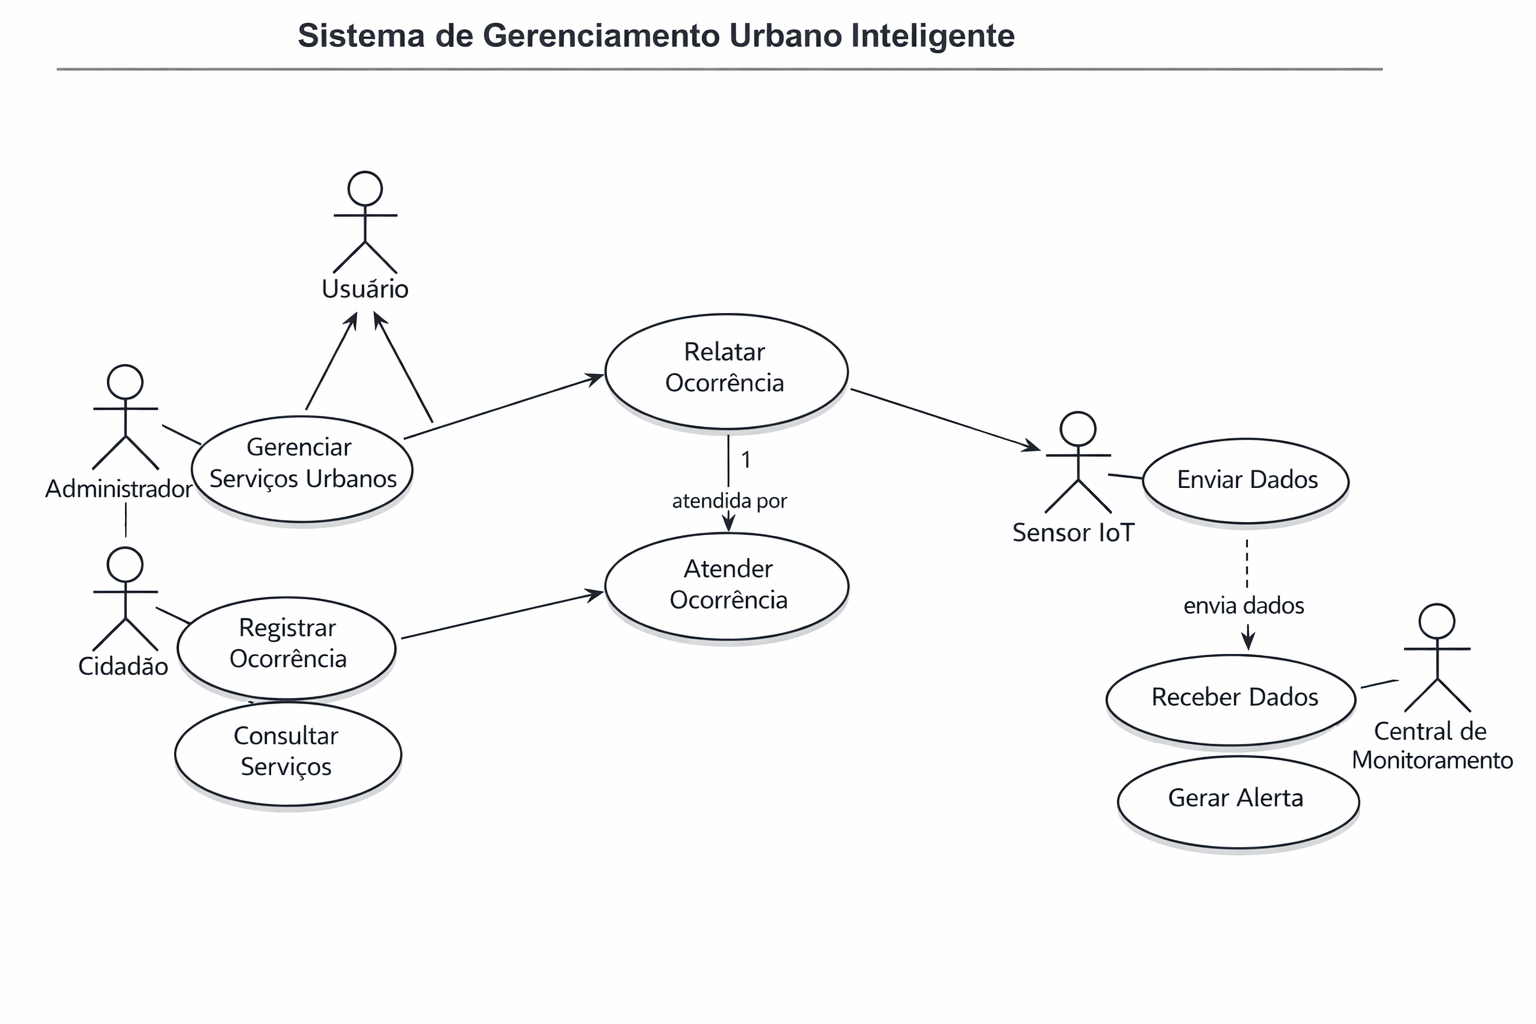
\includegraphics[width=0.8\textwidth]{images/diagramas/diagrama_de_casos_de_uso.png}
\label{fig:diagrama_de_casos_de_uso}
\end{figure}

\subsection{Requisitos}

\subsubsection{Requisitos Funcionais (RF)}

\begin{itemize}
  \item \textbf{RF01:} O sistema deve exibir dashboards integrados com indicadores de ocupação territorial e mobilidade.
  
  \item \textbf{RF02:} O sistema deve permitir a visualização de camadas de dados urbanos em um mapa de Aracaju.
  
  \item \textbf{RF03:} O sistema deve fornecer ferramentas para a simulação de cenários de intervenção urbana.
\end{itemize}

\subsubsection{Requisitos Não-Funcionais (RNF)}

\begin{itemize}
  \item \textbf{RNF01:} A interface deve ser otimizada para a tomada de decisão gerencial, com visualização de dados consolidada.
  
  \item \textbf{RNF02:} O sistema deve garantir a integração de dados provenientes de diferentes departamentos municipais.
\end{itemize}

\subsection{Telas do Sistema}

\begin{figure}[H]
\centering
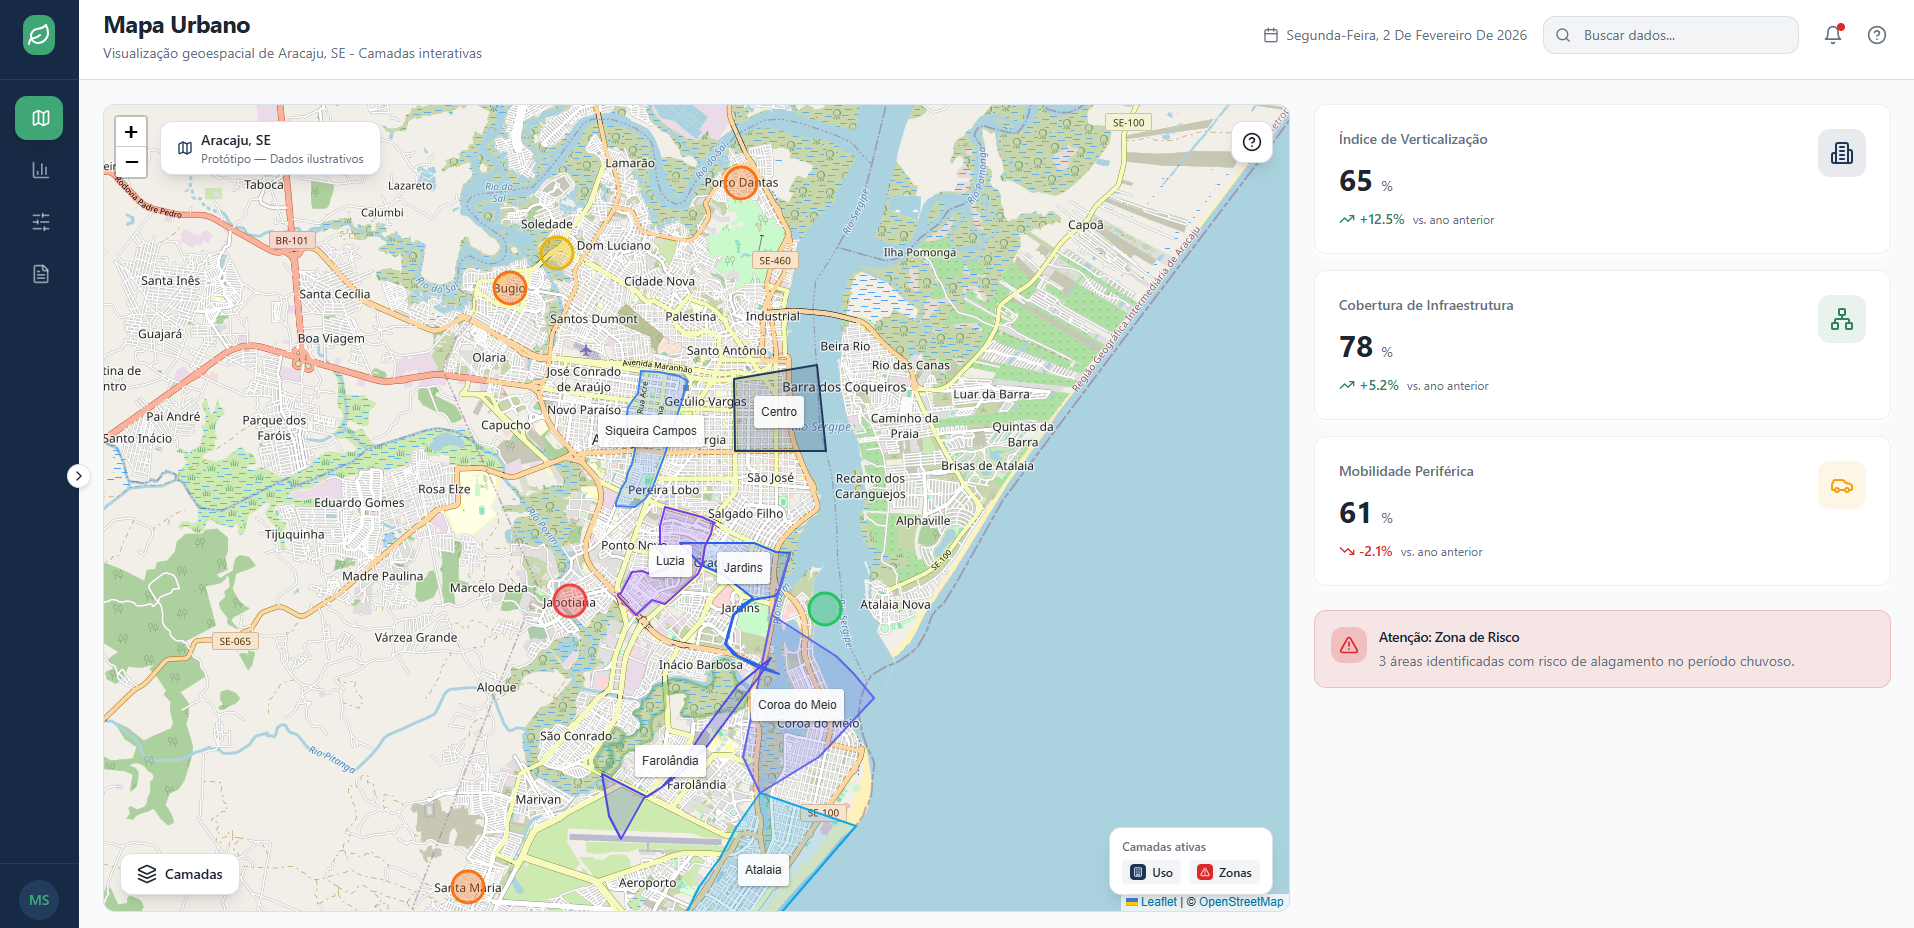
\includegraphics[width=0.9\textwidth]{images/dashboard_principal.png}
\caption{Dashboard principal do \textbf{MangueSMART}. Mapa urbano interativo com camadas de dados geoespaciais e indicadores de urbanização, infraestrutura e mobilidade.}
\label{fig:dashboard_principal}
\end{figure}

\begin{figure}[H]
\centering
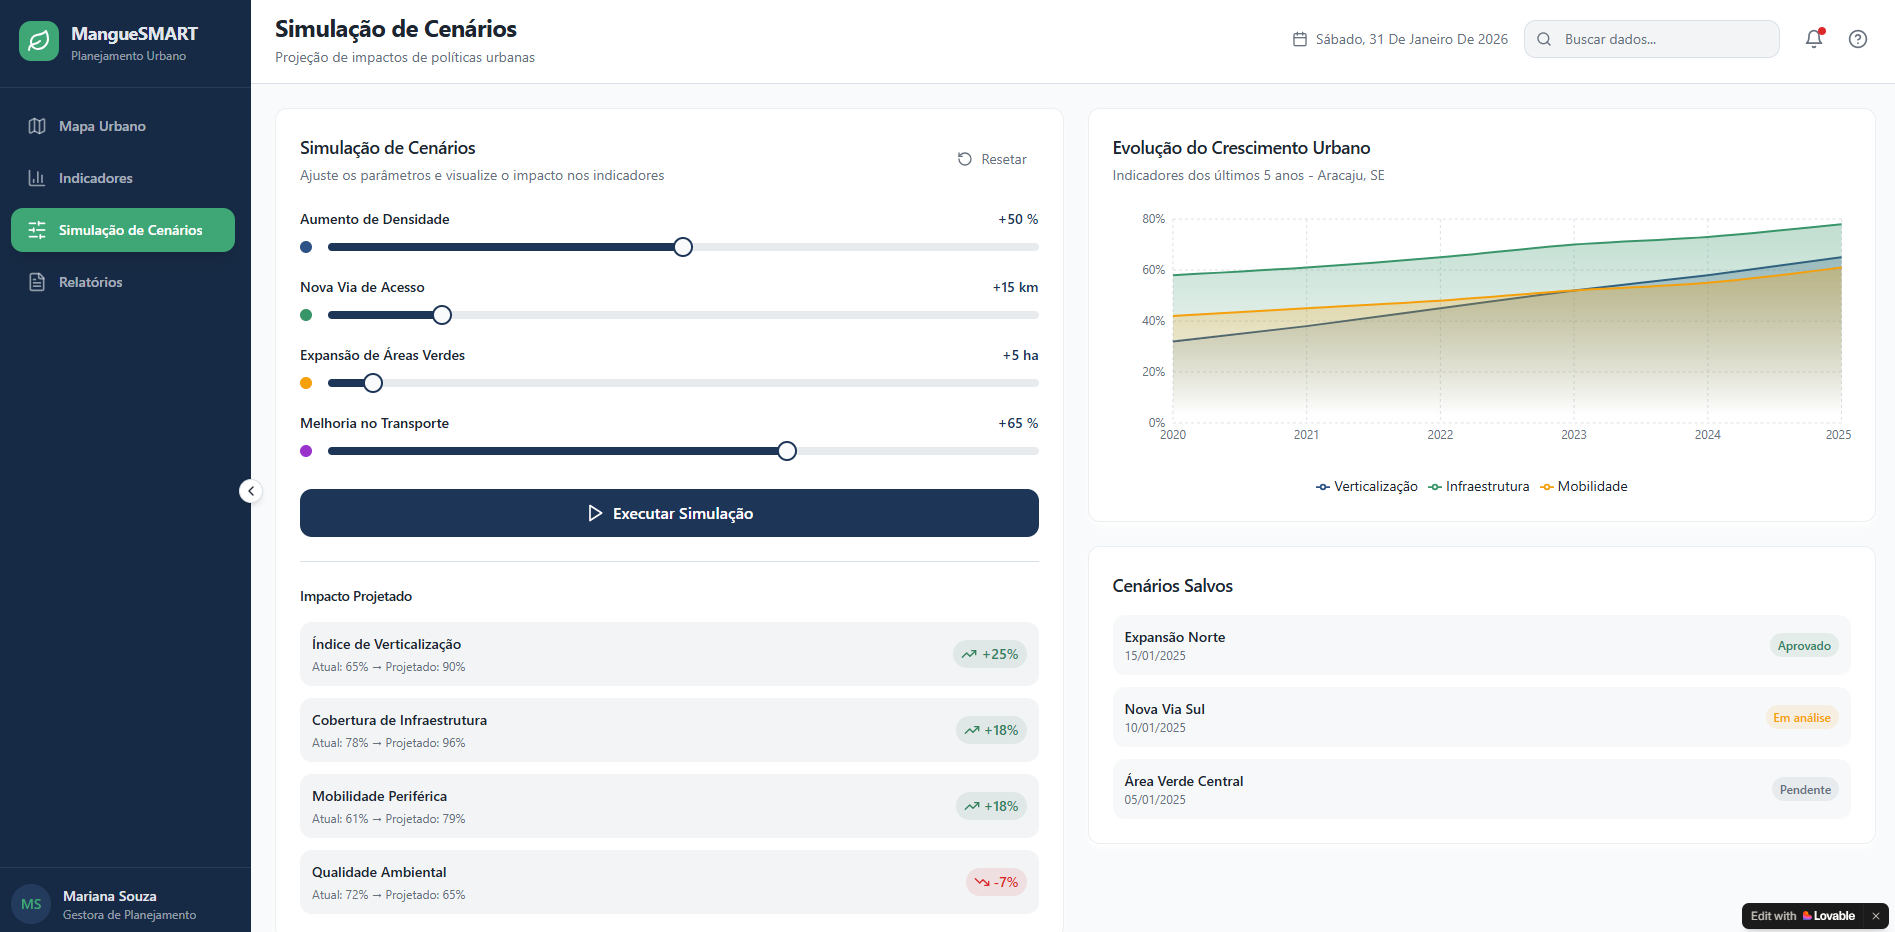
\includegraphics[width=0.9\textwidth]{images/simulacao_cenario.png}
\caption{Interface de simulação de cenários de intervenção urbana.}
\label{fig:simulacao_cenario}
\end{figure}

\begin{figure}[H]
\centering
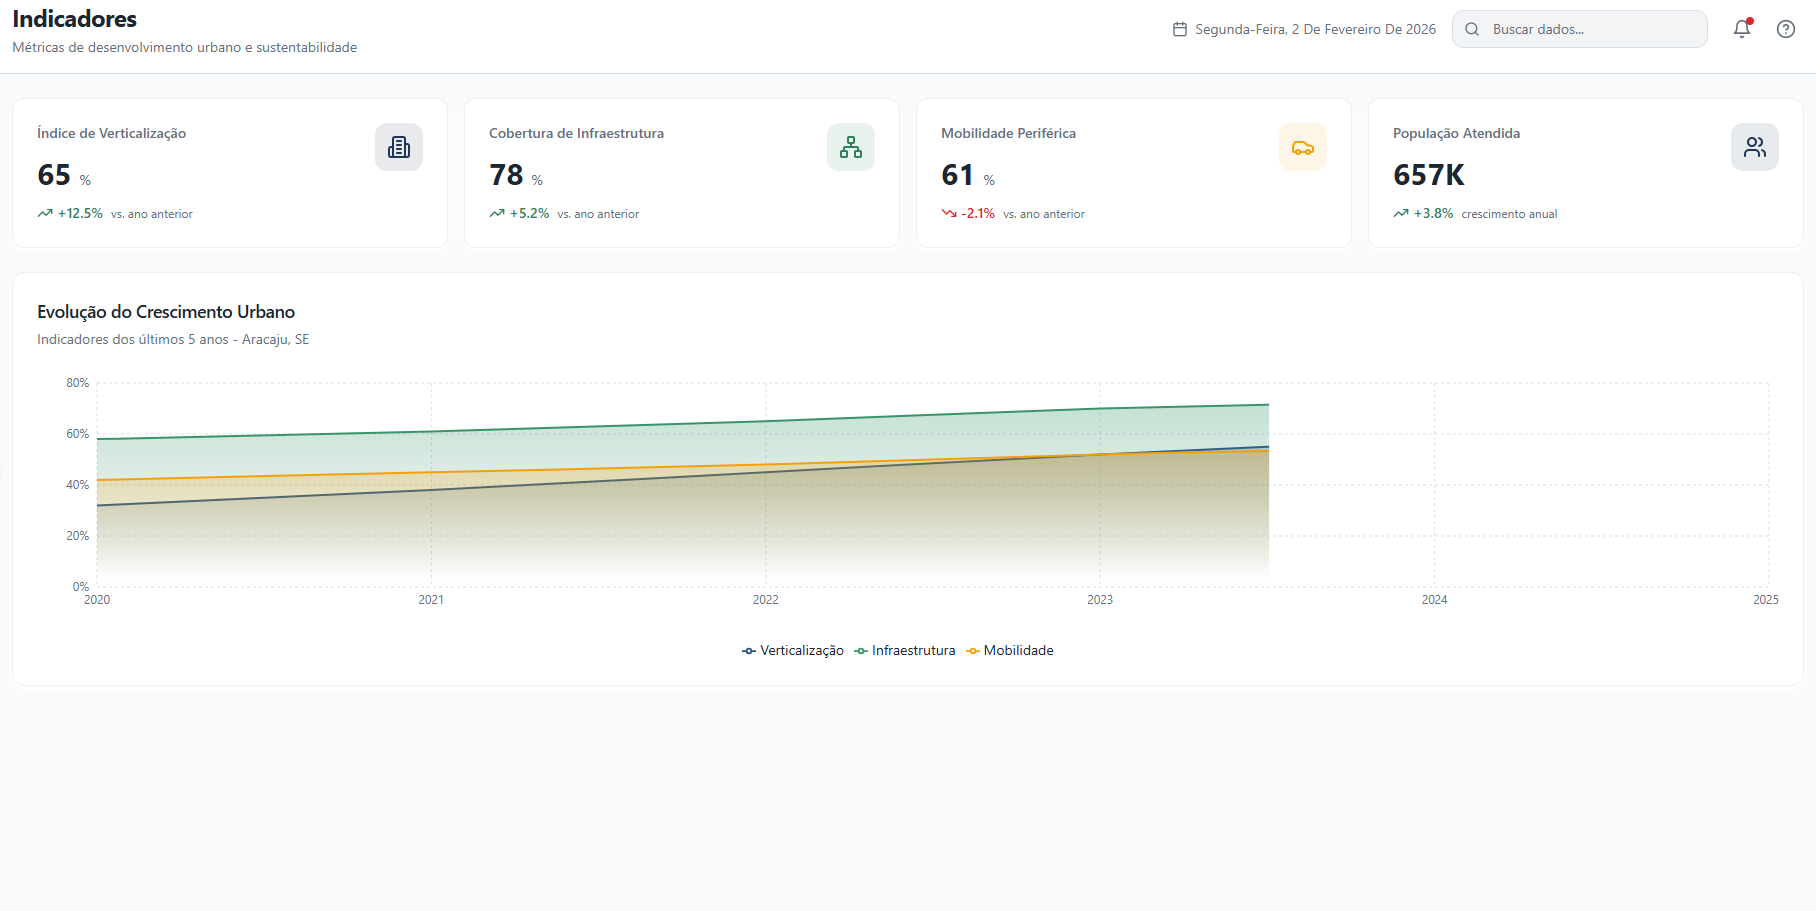
\includegraphics[width=0.9\textwidth]{images/indicadores.png}
\caption{Painel de indicadores com métricas de desenvolvimento urbano e gráfico de evolução do crescimento de Aracaju.}
\label{fig:indicadores}
\end{figure}

\begin{figure}[H]
\centering
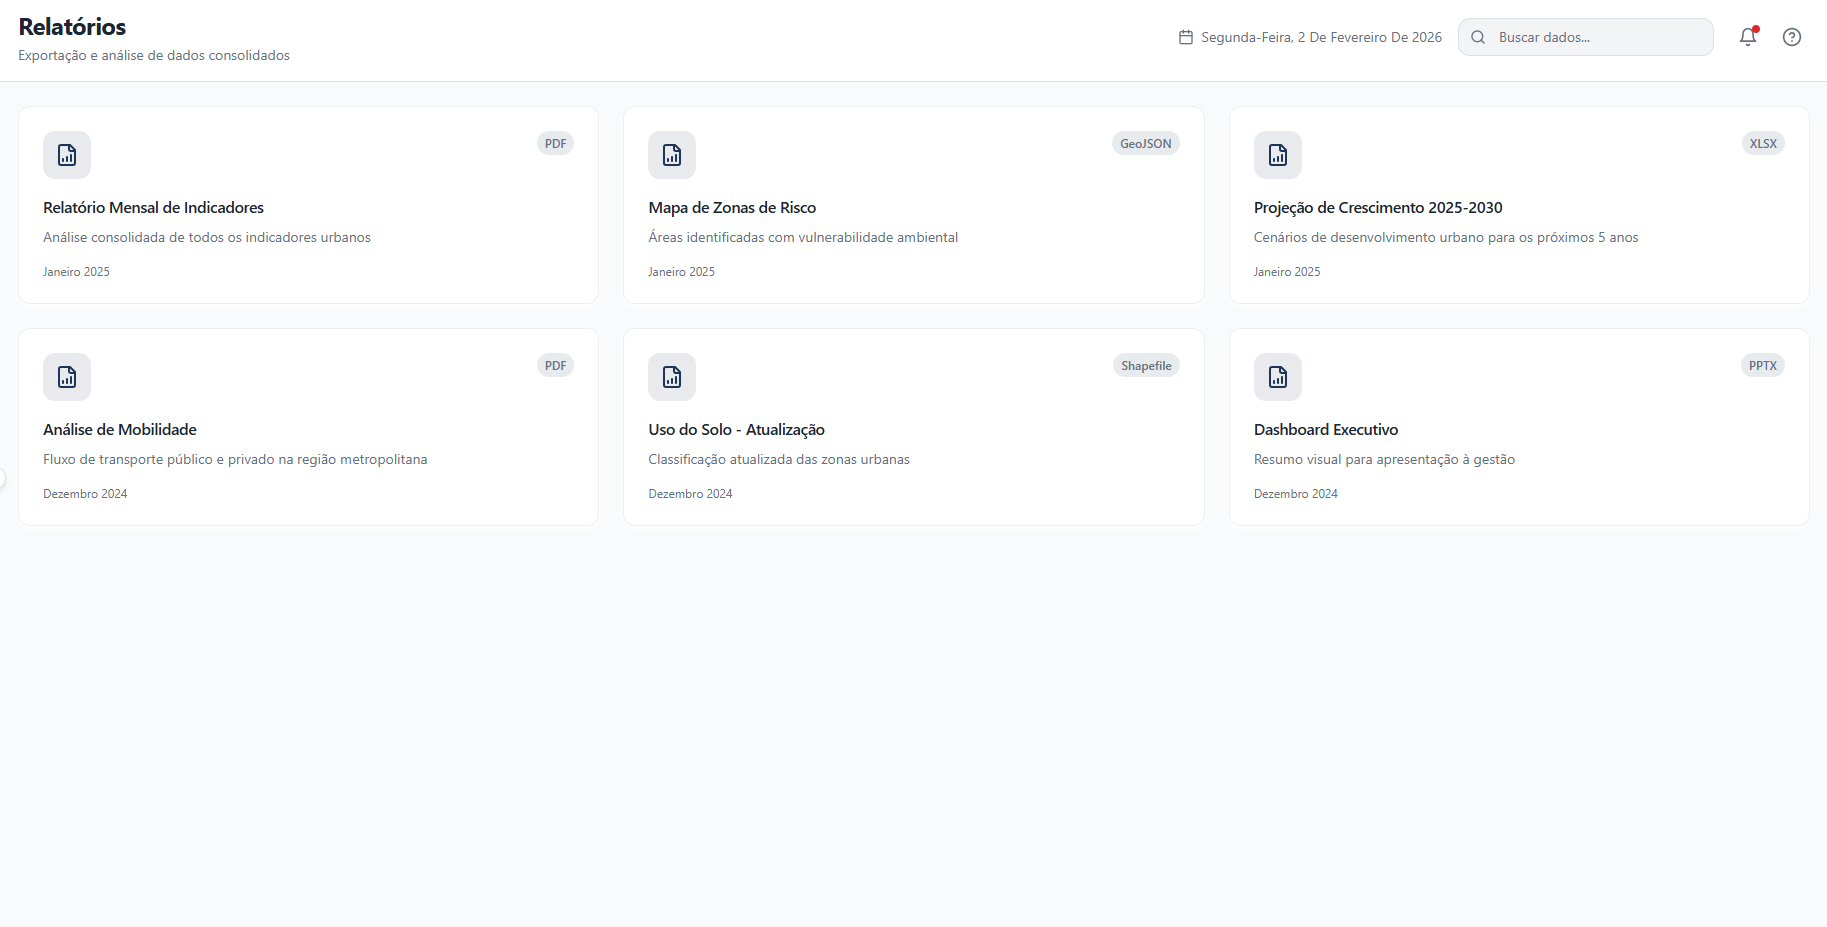
\includegraphics[width=0.9\textwidth]{images/relatorios.png}
\caption{Tela de relatórios para exportação e análise de dados consolidados em múltiplos formatos.}
\label{fig:relatorios}
\end{figure}

\begin{figure}[H]
\centering
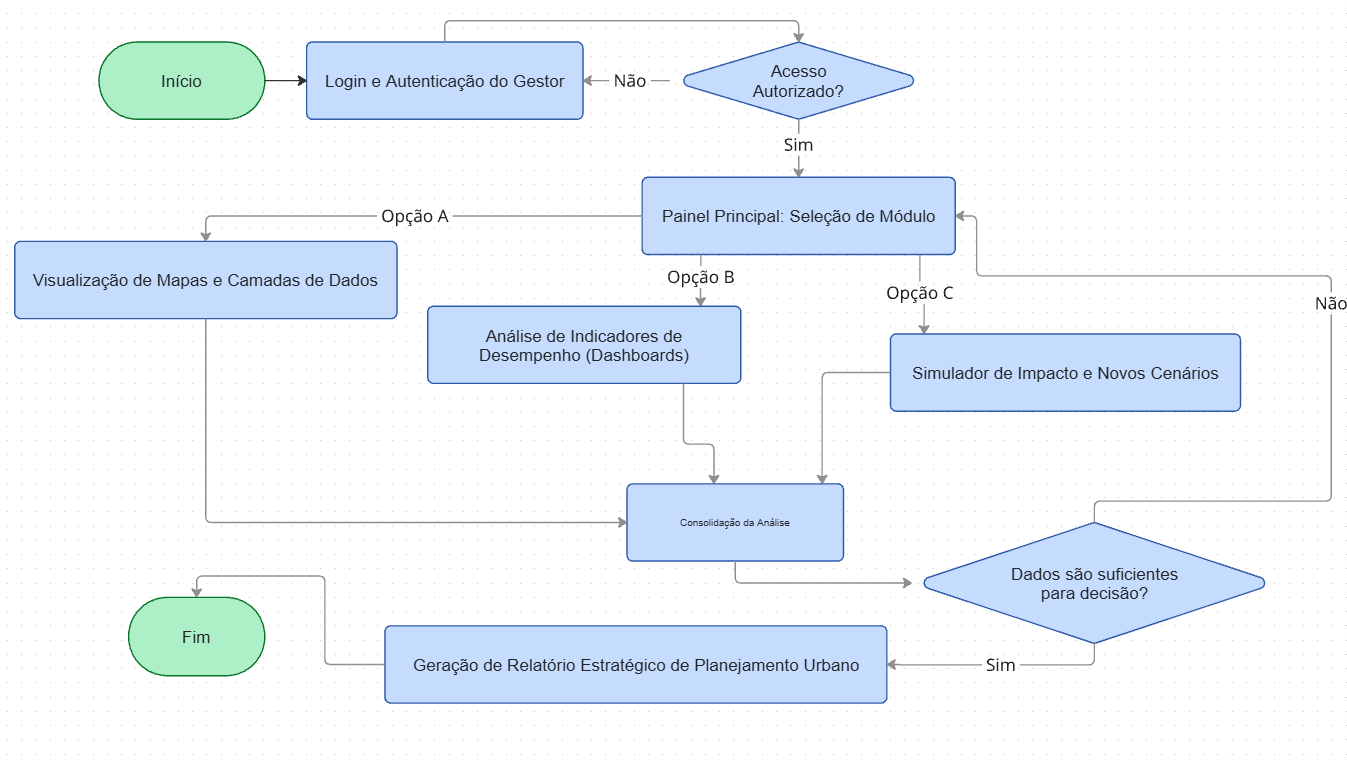
\includegraphics[width=0.9\textwidth]{images/fluxograma_manguesmart.png}
\caption{Fluxograma do Processo de Decisão no Sistema MangueSMART.}
\label{fig:fluxograma_manguesmart}
\end{figure}


\section{Quem fará o projeto}\label{sec:quem}

A execução e validação do projeto envolvem uma estrutura colaborativa entre a academia, o setor público e a equipe de desenvolvimento.

\subsection{Persona (Cliente-Alvo)}
O sistema é desenhado para atender às necessidades de gestores públicos, representados pela ``Persona'' Mariana Souza, Diretora de Planejamento Urbano. O foco é resolver a fragmentação de dados que dificulta a análise de impactos urbanos, como os observados na expansão da capital sergipana \cite{observatorio2023}. O objetivo é fornecer uma plataforma que permita simulações para garantir um crescimento ordenado.

\subsection{Stakeholders e Parcerias}
O projeto articula parcerias estratégicas com a Academia e órgãos estaduais, alinhando-se a iniciativas governamentais de revitalização e desenvolvimento urbano \cite{govse2025}. Os \textit{stakeholders} incluem a Secretaria de Planejamento (SEPLAN) e órgãos municipais (SMTT, EMURB), que atuarão na validação dos dados e da solução proposta.

\subsubsection{Mapa de Empatia do Tomador de Decisão}

Para compreender profundamente as necessidades e fricções vivenciadas pelo usuário final durante o processo de planejamento urbano, foi elaborado o Mapa de Empatia da persona ``Mariana Souza'' (Figura~\ref{fig:mapa_empatia}). Esta ferramenta permite alinhar as funcionalidades do \textit{MangueSMART} às expectativas reais de quem decide.

\begin{figure}[H]
\centering
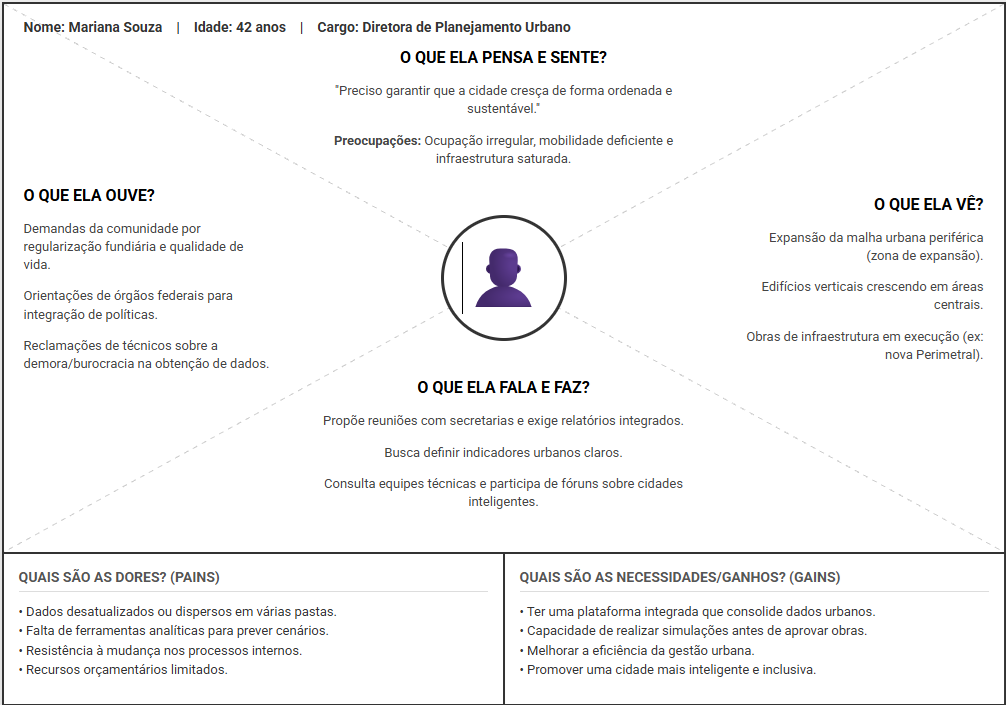
\includegraphics[width=0.9\textwidth]{images/mapa_empatia.png}
\caption{Mapa de Empatia da Persona Gestora (Mariana Souza).}
\label{fig:mapa_empatia}
\end{figure}

A análise do mapa revela que, embora a gestora tenha uma visão clara da necessidade de crescimento sustentável (``Pensa e Sente''), ela é bloqueada por obstáculos operacionais. O Quadro~\ref{quadro:empatia} detalha os principais pontos levantados.

\begin{table}[H]
\centering
\caption{Detalhamento das Dores e Necessidades da Persona.}
\label{quadro:empatia}
\begin{tabular}{@{}p{3cm} p{9.5cm}@{}}
\toprule
\textbf{Dimensão} & \textbf{Descrição} \\
\midrule
\textbf{O que ela vê?} & Expansão desordenada da malha urbana periférica, verticalização em áreas centrais e obras de infraestrutura em execução. \\
\midrule
\textbf{O que ela ouve?} & Demandas da comunidade por regularização fundiária, orientações federais e reclamações de técnicos sobre a demora na obtenção de dados. \\
\midrule
\textbf{Dores (Pains)} & Dados desatualizados ou dispersos entre secretarias; falta de ferramentas analíticas integradas; resistência interna à mudança de processos; recursos orçamentários limitados. \\
\midrule
\textbf{Ganhos (Gains)} & Acesso a uma plataforma integrada para simulação de cenários; melhoria na eficiência da gestão urbana; promoção de uma cidade inteligente, inclusiva e sustentável. \\
\bottomrule
\end{tabular}
\end{table}

Com base nesse mapeamento, o \textit{MangueSMART} foi projetado para atuar diretamente nas ``Dores'' identificadas, oferecendo a centralização de dados (resolvendo a dispersão) e dashboards de simulação (mitigando a falta de ferramentas analíticas), transformando as demandas de ``O que ela ouve'' em ações concretas de ``O que ela faz''.


\subsection{Equipe}

\begin{itemize}
  \item Beathriz Laurent Carlos Muniz: Coesão e coerência textual do artigo, elaboração do resumo e abstract, construção da introdução e conclusões, além da revisão final e padronização do documento em LaTeX;
  \item Jeferson de Oliveira Santos: Embasamento teórico do trabalho, levantamento e análise de trabalhos relacionados, definição da metodologia e premissas adotadas, descrição das limitações do projeto e organização das referências bibliográficas (.bib);
  \item João Marcos Peixoto Cavalcante: Definição da arquitetura de software do projeto, elaboração dos diagramas e descrição das visões arquiteturais (lógica, desenvolvimento, processo, física e casos de uso), garantindo a viabilidade técnica da solução proposta;
  \item Marcelo Pedral Mota: Análise de requisitos, prototipagem de interface (UX/UI), definição do escopo do produto e cronograma de entregas;
  \item Niceu Santos Biriba: Definição da justificativa do projeto sob a ótica de negócio, análise dos benefícios, identificação dos stakeholders, elaboração do mapa de empatia, análise de custos, riscos e viabilidade do projeto;
  \item Gilton José Ferreira da Silva: Coordenação do trabalho, correções e direcionamentos da pesquisa.
\end{itemize}

\section{Como o projeto será feito?} \label{sec:Como}

A metodologia adotada para o desenvolvimento do MangueSMART caracteriza-se como uma pesquisa de natureza aplicada e tecnológica, visando a construção de um protótipo funcional (Produto Mínimo Viável - MVP) de um Sistema de Apoio à Decisão (SAD). O processo foi estruturado em três fases distintas: Concepção e Planejamento, Modelagem Arquitetural e Desenvolvimento do Protótipo/Validação \cite{SAD2025}.

\subsection{Premissas}
O desenvolvimento do sistema parte da premissa da disponibilidade de dados abertos governamentais ou amostras fornecidas pelas secretarias parceiras (SEPLOG, SMTT), conforme identificado na fase de concepção. Assume-se também o acesso contínuo aos stakeholders chave ("Persona Mariana Souza") para validações quinzenais das funcionalidades do MVP.

\subsection{Grupo de entregas}
As principais entregas do projeto estão alinhadas aos ciclos de desenvolvimento detalhados na Tabela \ref{tab:cronograma}. O conjunto de artefatos inclui:
\begin{itemize}
    \item \textbf{Planejamento:} Project Model Canvas e Documento de Requisitos.
    \item \textbf{Dados:} Base de dados geoespaciais padronizada com camadas de uso do solo e mobilidade.
    \item \textbf{Software:} Protótipo funcional (MVP) composto por Dashboards de indicadores e Mapa Urbano Interativo.
    \item \textbf{Análise:} Módulo de simulação de cenários de intervenção urbana e gerador de relatórios estratégicos.
\end{itemize}

\subsection{Restrições}
O desenvolvimento do MangueSMART enfrenta limitações que delimitam o alcance do MVP:
\begin{itemize}
    \item \textbf{Tecnológica:} O projeto foca exclusivamente no desenvolvimento de uma aplicação \textit{Web}, não contemplando versões \textit{mobile} nativas nesta fase.
    \item \textbf{Dados:} A precisão do sistema é condicionada à qualidade dos dados abertos fornecidos pela prefeitura; a defasagem do Plano Diretor de Desenvolvimento Urbano (PDDU) pode gerar discrepâncias nas simulações legais.
    \item \textbf{Científica:} O módulo de simulação atua como uma Prova de Conceito, simplificando variáveis microclimáticas e hidrológicas complexas.
    \item \textbf{Operacional:} A validação técnica foi realizada com um grupo restrito de \textit{stakeholders}, sem a execução de testes de carga em larga escala.
\end{itemize}

\section{Quando e quanto?} \label{sec:quandoquanto}

\subsection{Gerenciamento de Riscos}
O projeto mitiga riscos técnicos e organizacionais, como a desatualização de dados públicos e a resistência interna à mudança. A estratégia envolve validações constantes e a adoção de indicadores consolidados na literatura de cidades inteligentes \cite{iwasa2025} para garantir a robustez das decisões.

\subsection{Linha do tempo}

O desenvolvimento do \textbf{MangueSMART} foi estruturado em cinco etapas iterativas, conforme apresentado na Tabela~\ref{tab:cronograma}. A organização em ciclos curtos permitiu entregas incrementais, começando pelo levantamento e modelagem dos dados urbanos de Aracaju e evoluindo até a validação do MVP com stakeholders.

\begin{table}[H]
\centering
\caption{Cronograma de desenvolvimento do projeto MangueSMART.}
\label{tab:cronograma}
\begin{tabular}{@{}p{2.2cm} p{3cm} p{7cm}@{}}
\toprule
\textbf{Período} & \textbf{Fase} & \textbf{Principais Entregas} \\
\midrule
Semanas 1--2 & Concepção e Planejamento & Definição do Project Model Canvas, levantamento de requisitos com stakeholders (SEPLAN, SMTT) e identificação das fontes de dados urbanos. \\
Semanas 3--4 & Aquisição e Modelagem de Dados & Coleta e padronização dos dados geoespaciais (uso do solo, zonas de risco, mobilidade) e definição da arquitetura do sistema. \\
Semanas 5--7 & Desenvolvimento do MVP & Construção dos dashboards de indicadores, mapa urbano interativo com camadas de dados e módulo de relatórios. \\
Semanas 8--9 & Simulação e Integração & Implementação da interface de simulação de cenários de intervenção urbana e integração dos módulos em uma plataforma unificada. \\
Semanas 10--12 & Validação e Ajustes & Testes de usabilidade com a persona gestora, validação dos indicadores junto aos órgãos municipais e ajustes finais do protótipo. \\
\bottomrule
\end{tabular}
\end{table}

\subsection{Custos}

A estimativa de custos do \textbf{MangueSMART} considera uma equipe de 5 profissionais atuando durante o ciclo de 12 semanas, com infraestrutura adequada para um sistema em ambiente de produção. A Tabela~\ref{tab:custos} apresenta o detalhamento dos custos projetados.

\begin{table}[H]
\centering
\caption{Estimativa de custos do projeto MangueSMART (12 semanas).}
\label{tab:custos}
\begin{tabular}{@{}p{5.5cm} p{2.5cm} p{3.5cm}@{}}
\toprule
\textbf{Item} & \textbf{Frequência} & \textbf{Custo Estimado} \\
\midrule
Equipe de desenvolvimento (5 profissionais júnior) & Mensal & R\$ 22.500/mês \\
Infraestrutura de nuvem (servidores, banco de dados, CDN) & Mensal & R\$ 1.000/mês \\
Serviços de dados geoespaciais (APIs de mapas e geocodificação) & Mensal & R\$ 150/mês \\
Licenças de software (ferramentas de BI, monitoramento, CI/CD) & Mensal & R\$ 400/mês \\
Domínio e certificado SSL & Anual & R\$ 100/ano \\
\midrule
\textbf{Total estimado (3 meses)} & & \textbf{R\$ 72.250} \\
\bottomrule
\end{tabular}
\end{table}

O financiamento prevê o aproveitamento de editais de inovação e convênios federais voltados para modernização urbana e regularização fundiária \cite{agenciagov2025}. A maior parcela dos custos concentra-se na remuneração da equipe, o que reforça a importância de parcerias institucionais e fontes de financiamento público para viabilizar o projeto em escala real.


\section{Limitações do Trabalho} \label{sec:ameacas}

Embora o desenvolvimento do protótipo funcional (MVP) do sistema MangueSMART tenha alcançado os objetivos propostos de integração e visualização de dados urbanos, este trabalho apresenta limitações inerentes ao seu escopo acadêmico e às restrições técnicas e operacionais identificadas durante o processo.

A primeira limitação refere-se à disponibilidade e qualidade dos dados primários. O sistema opera sob a premissa da existência de dados abertos e estruturados fornecidos pela administração municipal. No entanto, conforme apontado por Santos (2024), plataformas digitais preexistentes, como o AjuInteligente, muitas vezes funcionam apenas como digitalizadores de processos burocráticos, sem necessariamente prover bases de dados analíticas integradas ou dados estruturados em tempo real \cite{Santos2024}. Adicionalmente, a defasagem do Plano Diretor de Desenvolvimento Urbano (PDDU), cuja última grande atualização ocorreu em 2000, conforme destacado por Meneses et al. (2024), impõe um desafio à precisão das simulações de cenários legais, uma vez que as regras de ocupação do solo cadastradas no sistema podem não refletir a dinâmica atual da expansão urbana e das áreas de risco \cite{Meneses2024}.

Em relação ao escopo técnico e de plataforma, o projeto limitou-se ao desenvolvimento de uma aplicação \textit{Web}, não contemplando, nesta fase, uma versão \textit{mobile} nativa, o que restringe a usabilidade em campo por agentes que necessitem de acesso via dispositivos móveis em áreas sem conectividade estável \cite{SAD2025}. Além disso, o módulo de simulação de cenários focou na demonstração de viabilidade técnica (Prova de Conceito) com um número reduzido de variáveis, não abarcando a totalidade de complexidades hidrológicas e climáticas necessárias para uma modelagem preditiva de alta precisão, como as variações microclimáticas detalhadas por Santos e Pinto (2020) que exigiriam séries temporais históricas mais robustas \cite{SantosPinto2020}. 

Por fim, restrições orçamentárias e de cronograma acadêmico limitaram a validação do sistema a um grupo restrito de \textit{stakeholders}. A implementação de testes de carga em larga escala, bem como a auditoria completa de segurança da informação e adequação a todos os preceitos da Lei Geral de Proteção de Dados (LGPD) em ambiente de produção, foram identificadas como riscos e atividades futuras, não sendo exauridas no presente trabalho \cite{SAD2025}.


\section{Considerações Finais} \label{sec:consideracoes}
O desenvolvimento do MangueSMART demonstrou ser uma solução viável para superar a fragmentação de dados na gestão pública de Aracaju, permitindo uma transição para o planejamento orientado por dados (data-driven). Embora o protótipo tenha validado a integração de indicadores e a simulação de cenários, o sucesso a longo prazo depende da atualização das bases de dados municipais e da modernização do Plano Diretor. Atividades futuras incluem a implementação de testes de carga, auditoria de segurança conforme a LGPD e o desenvolvimento de módulos preditivos mais robustos.

\section*{Agradecimentos} \label{sec:agradecimentos}

Esta seção é reservada para expressar gratidão às instituições e indivíduos que apoiaram a pesquisa, como a Universidade Federal de Sergipe (UFS), a Secretaria de Planejamento de Aracaju (SEPLAN) e os membros da equipe de desenvolvimento.






\bibliographystyle{sbc}
\bibliography{referencias}


\end{document}
